\begin{section}{Including next nearest neighbor hopping}

\label{section3NNN}

In the previous sections we have seen that the second order perturbation effective Hamiltonian will contain the following terms:

\begin{itemize}
	\item Exchange interaction $J_{ij} \bs{S}_i \bs{S}_j$, arising from the kinetic hopping - kinetic hopping terms.
	\item DMI $\bs{D}_{ij} \bs{S}_i \times \bs{S}_j$, arising from the kinetic hopping - SOI hopping terms.
	\item Anisotropic or pseudodipolar interaction $\bs{S}_i \bs{\Gamma}_{ij} \bs{S}_j$, arising from the SOI hopping - SOI hopping terms.
\end{itemize}

And all these coupling factors will be renormalized by the laser field. This renormalization depends only on the field and the sites $i$, $j$, it does not depend on the nature of the interaction. With this in mind we will introduce a model with additional NNN hopping terms: 

\begin{equation}
\label{BigHam}
\hat{H} = -\sum_{\langle i,j \rangle, \sigma, \sigma'}(\delta_{\sigma, \sigma'} t_1 + \bs{\Delta}_{1,ij}\cdot \bs{\sigma}_{\sigma, \sigma'})\hat{c}_{i \sigma}^\dagger \hat{c}_{j \sigma'} - 
	\sum_{\langle \langle i,j \rangle \rangle, \sigma, \sigma'}(\delta_{\sigma, \sigma'} t_2 + \bs{\Delta}_{2,ij}\cdot \bs{\sigma}_{\sigma, \sigma'})\hat{c}_{i \sigma}^\dagger \hat{c}_{j \sigma'} + 
	\text{U}\hat{D}
\end{equation}

Where sum over next-nearest neighbors is denoted by $\langle \langle i j \rangle \rangle$. This Hamiltonian is the same we studied in section \ref{Section3HubbardSOI} plus a NNN hopping and SOI term. The hopping amplitudes thus are:

\begin{equation}
\label{BigHamHoppingAmp}
t_{ij}^{\sigma \sigma'} = \begin{cases}
	(\delta_{\sigma \sigma'}t_1+\bs{\Delta}_{1,ij}\cdot \bs{\sigma}_{\sigma, \sigma'}) & \text{for } i, j \text{ nearest neighbors} \\
	(\delta_{\sigma \sigma'}t_2+\bs{\Delta}_{2,ij}\cdot \bs{\sigma}_{\sigma, \sigma'}) & \text{for } i, j \text{ next nearest neighbors} \\
	0 & \text{ otherwise}
\end{cases} \quad
\end{equation}

The effective Hamiltonian will be the same as in section \ref{Section3HubbardSOI}, with the corresponding NNN terms. This is because in second order perturbation NN hopping terms do not mix with NNN hopping terms. Thus, the effective spin Hamiltonian will be:

\begin{align}
\hat{H}_{\text{eff}}(t) = &\sum_{\langle i,j \rangle} \left\{ J_{1,ij}\bs{S}_i\cdot\bs{S}_j + \bs{D}_{1,ij} \cdot\bs{S}_i \times \bs{S}_j + \bs{S}_i\bs{\Gamma}_{1,ij}\bs{S}_j\right\} + \nonumber \\
&\sum_{\langle \langle i,j \rangle \rangle} \left\{ J_{2,ij}\bs{S}_i\cdot\bs{S}_j + \bs{D}_{2,ij}\cdot \bs{S}_i \times \bs{S}_j + \bs{S}_i\bs{\Gamma}_{2,ij}\bs{S}_j\right\}
\end{align}

Where:

\begin{align}
J_{n,ij} &= t_n^2\mathcal{M}(\alpha_{ij}, \text{U}, \omega, t) \label{JGeneral} \\
\bs{D}_{n,ij} &= 2it_n \bs{\Delta}_{n,ij}\mathcal{M}(\alpha_{ij}, \text{U}, \omega, t) \label{DGeneral} \\
\Gamma_{n,ij}^{\alpha \beta} &= (\delta_{\alpha \beta} \bs{\Delta}_{n,ij}^2 - 2\Delta_{n,ij}^\alpha\Delta_{n,ij}^\beta )\mathcal{M}(\alpha_{ij}, \text{U}, \omega, t) \label{GammaGeneral}
\end{align}

NNN interaction coupling factors will be normalized according to $\mathcal{M}(\alpha_{ij}, \text{U}, \omega, t)$, where $i$, $j$ are NNN sites, whereas NN interaction coupling factors will be normalized according to $\mathcal{M}(\alpha_{ij}, \text{U}, \omega, t)$ where $i$, $j$ are NN sites. Therefore the dependence on the field will differ. For example, if we take the time independent approximation \ref{MFactorApprox}, and use $\lambda = \pm 1$ for circular polarized light, and $\alpha_{ij} = \pm\frac{\mathcal{E}|\bs{R}_{ij}|}{a\sqrt{2}}$, where $\mathcal{E} = \frac{eaE_0}{\omega}$. Then the exchange interaction will be:

\begin{align*}
J_{1,ij} &= J_1^0 + t_1^2 \frac{\mathcal{E}^2}{2} \left( \frac{1}{\text{U}+\omega} + \frac{1}{\text{U}-\omega} \right) = J_1^0 + J_1^0 \frac{\mathcal{E}^2}{2} \left( \frac{1}{1+\frac{\omega}{\text{U}}} + \frac{1}{1-\frac{\omega}{\text{U}}} \right) \\
J_{2,ij} &= J_2^0 + t_2^2 \frac{3\mathcal{E}^2}{2} \left( \frac{1}{\text{U}+\omega} + \frac{1}{\text{U}-\omega} \right) = J_2^0 + J_2^0 \frac{3\mathcal{E}^2}{2} \left( \frac{1}{1+\frac{\omega}{\text{U}}} + \frac{1}{1-\frac{\omega}{\text{U}}} \right) \\
\end{align*}

Where $J_n^0 = \frac{t_n^2}{\text{U}}$ and where we used that $|\bs{R}_{ij}| = a$ for NN and $|\bs{R}_{ij}| = \sqrt{3}a$ for NNN in a honeycomb lattice. The other coupling factors in \ref{DGeneral} and \ref{GammaGeneral} can be approximated in the same way.

In section \ref{Numerics} we will investigate this numerically. The reason why the renormalization differs for NN and NNN spin interactions is that in a hopping process, the electron picks up a phase $e^{ie\bs{R}_{ij}\cdot\bs{A}(t)}$ (assuming flat field approximation). This phase will be larger for NNN hopping than for NN hopping and this will therefore translate in the corresponding spin interactions.

Next we will show several well-known models which are described by \ref{BigHam}.

\begin{subsection}{Kane-Mele-Hubbard model}

The first model to describe topological insulators was introduced by Kane and Mele \cite{Kane2005} to describe quantum spin Hall effect in graphene. In a honeycomb lattice time reversal symmetry and inversion symmetry allow only next-nearest neighbor spin orbit coupling, which is known as intrinsic spin orbit coupling. In these circumstances the system can be modeled by the Kane-Mele-Hubbard model:

\begin{align}
\label{KMH}
\hat{H}_{\text{KMH}} &= -t_1\sum_{\langle i j \rangle \sigma} \hat{c}^{\dagger}_{i\sigma}\hat{c}_{j\sigma} + i\Delta \sum_{\langle \langle i j \rangle \rangle \sigma \sigma'} \hat{c}^{\dagger}_{i\sigma} \nu_{ij} \sigma^z_{\sigma \sigma'} \hat{c}_{j\sigma'} + \text{U}\hat{D}
\end{align}
Where $\Delta$ is the intrinsic spin orbit coupling constant. $\nu_{ij}=\pm 1$ depending on whether the electron traversing from $i$ to $j$ makes a right ($+1$) or a left turn ($-1$). This Hamiltonian is described by \ref{BigHam} if we set $\bs{\Delta}_{1,ij} = 0$, $t_2 = 0$ and $\bs{\Delta}_{2,ij} = -i\Delta \nu_{ij} \hat{e}_z$. Then, the effective spin model will be:

\begin{equation}
\label{KMHeff}
\hat{H}_{\text{KMH}}^{\text{eff}}(t) = \sum_{\langle i,j \rangle} J_{ij} \bs{S}_i \cdot\bs{S}_j + \sum_{\langle \langle i,j \rangle \rangle} \bs{S}_i \bs{\Gamma}_{ij} \bs{S}_j 
\end{equation}
With and:

\begin{align*}
J_{ij} &= t_1^2\mathcal{M}(\alpha_{ij}, \text{U}, \omega, t) \\
\bs{\Gamma}_{ij} &= \Delta^2 \text{diag}(-1,-1,1)\mathcal{M}(\alpha_{ij}, \text{U}, \omega, t)
\end{align*}
according to \ref{JGeneral} and \ref{GammaGeneral}. Notice that:

\begin{equation*}
\bs{S}_i \bs{\Gamma}_{ij} \bs{S}_j = \Delta^2 \mathcal{M}(\alpha_{ij}, \text{U}, \omega, t) \left(S_i^zS_j^z - S_i^xS_j^x - S_i^yS_j^y\right)
\end{equation*}
This describes a type of anisotropic exchange interaction known as XXZ Heisenberg model for next nearest neighbors. Notice that the anisotropic term breaks the SU(2) symmetry of the bare Heisenberg model. The same spin model is obtained in \cite{Rachel2010} without the laser perturbation, this model has a much richer phase diagram than the $J_1-J_2$ Heisenberg model \cite{Vaezi2012}. If the laser field is not too strong so that we can assume $\mathcal{M}(\alpha_{ij}, \text{U}, \omega, t) > 0$, then $\Gamma^{zz}_{ij} > 0$. Therefore we see that this interaction favors antiferromagnetic order in the $\hat{e}_z$ direction and ferromagnetic order in the $\hat{e}_x-\hat{e}_y$ plane. The exchange interaction $J_{ij}$ will favor antiferromagnetic order for nearest neighbors, so that next nearest neighbors will tend to be aligned. Therefore, $\Gamma^{zz}_{ij}$ will compete against $J_{ij}$ in the $\hat{e}_z$ direction. In the $\hat{e}_x-\hat{e}_y$ plane, $\bs{\Gamma}_{ij}$ will favor ferromagnetic order between next nearest neighbors, which adds to the effect of $J_{ij}$. In general the strength of the exchange interaction will be larger and the net effect of $\bs{\Gamma}_{ij}$ will be a tilting of the spins towards the $\hat{e}_x$-$\hat{e}_y$ plane.

\end{subsection}

\begin{subsection}{Modified Kane-Mele-Hubbard model}

As we saw in the previous section the effective Hamiltonian \ref{KMHeff} does not contain NNN DMI terms. The reason for this is because in the original Hamiltonian $t_2 = 0$. Next we will study the same Hamiltonian adding a finite NNN hopping terms $t_2$. In general this is more accurate than imposing $t_2 = 0$, and it can be understood as a second order NN hopping process (the direct NNN hopping integral would usually be much smaller). Our next Hamiltonian is thus:

\begin{equation}
\label{MKMH}
\hat{H} = - t_1\sum_{\langle i,j \rangle, \sigma} \hat{c}_{i \sigma}^\dagger \hat{c}_{j \sigma} -
	\sum_{\langle \langle i,j \rangle \rangle, \sigma}(t_2 - i\Delta\nu_{ij}\sigma^z_{\sigma, \sigma})\hat{c}_{i \sigma}^\dagger \hat{c}_{j \sigma} + 
	\text{U}\hat{D}
\end{equation}
\begin{figure}
\centering
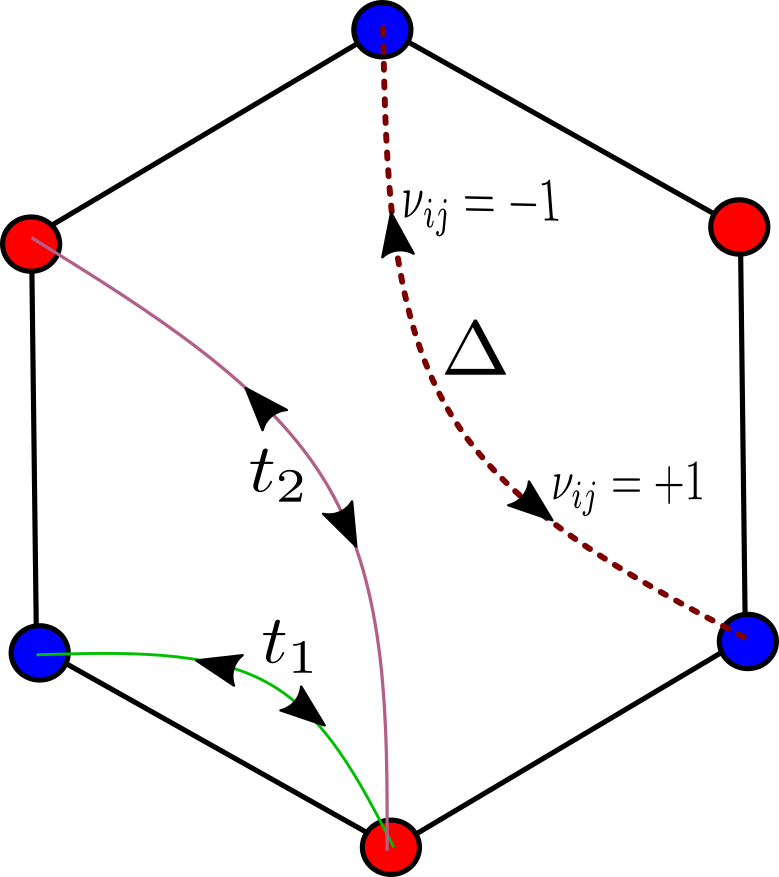
\includegraphics[width=0.5\columnwidth]{../Figures/kmh.png}
\caption{A honycomb cell with NN hopping $t_1$, NNN hopping $t_2$ and intrinsic SOI $\Delta$. $\nu_{ij} = \pm 1$ depending on whether the electron traversing from $i$ to $j$ makes a right ($+1$) or a left turn ($-1$).}
\label{fig:MKMH}
\vspace*{-6pt}
\end{figure}
This corresponds to the case $\bs{\Delta}_{1,ij} = 0$ and $\bs{\Delta}_{2,ij} = (0, 0, -i\nu_{ij} \Delta)$ in \ref{BigHam}. The Hamiltonian parameters are sketched in Figure \ref{fig:MKMH}. With this, the effective Hamiltonian will be:

\begin{equation}
\label{MKMHeff}
\hat{H}_{\text{eff}}(t) = \sum_{\langle i,j \rangle} J_{1,ij}\bs{S}_i\cdot\bs{S}_j + \sum_{\langle \langle i,j \rangle \rangle} \left\{ J_{2,ij}\bs{S}_i\cdot\bs{S}_j + \bs{D}_{2,ij}\cdot \bs{S}_i \times \bs{S}_j + \bs{S}_i \bs{\Gamma}_{ij} \bs{S}_j \right\}
\end{equation}
Where:

\begin{align*}
J_{1,ij} &= t_1^2\mathcal{M}(\alpha_{ij}, \text{U}, \omega, t) \\
J_{2,ij} &= t_2^2\mathcal{M}(\alpha_{ij}, \text{U}, \omega, t) \\
\bs{D}_{2,ij} &= 2\nu_{ij} t_2 \Delta \hat{e}_z \mathcal{M}(\alpha_{ij}, \text{U}, \omega, t) \\
\bs{\Gamma}_{2,ij} &= \Delta^2 \text{diag}(-1,-1,1) \mathcal{M}(\alpha_{ij}, \text{U}, \omega, t) 
\end{align*}
Such a Hamiltonian was first proposed by S. A. Owerre to model honeycomb topological magnon insulators \cite{Owerre2016} \cite{Elyasi2018}. Experimental results regarding topological properties of spin waves in honeycomb ferromagnet Cr$I_3$ can only be understood by considering this Hamiltonian \cite{Chen2018}. This model is also relevant for the study of Spin Hall effects of Weyl magnons \cite{Zyuzin2018} \cite{Sekine2016}.

Now, a Hamiltonian with the form $\hat{H} = \sum_{\langle i,j \rangle} J_1 \bs{S}_i\cdot\bs{S}_j + \sum_{\langle \langle i,j \rangle \rangle} J_2\bs{S}_i\cdot\bs{S}_j$ is known as the $J_1$-$J_2$ Heisenberg model and in a 2D honeycomb lattice it exhibits N\'eel order for $J_2 < J_1 / 6$ and for $J_2 > J_1 / 6$ spin density waves (SDW) appear \cite{Mulder2010}. In the presence of DMI alone there will always be SDW in the plane perpendicular to $\bs{D}$ \cite{Uchida2006}. In Hamiltonian \ref{MKMHeff} we expect SDW to appear in the ground state and the SDW wavevector will be determined by a function of the parameters of this model. In the next section we will do a numerical of study on how modifying the ratio between NN and NNN spin interaction factors can change the spin state of the system.

\end{subsection}

\begin{subsection}{Time independent electric field in the NN + NNN Hamiltonian}

Now, let us examine the case in which the applied electric field is time independent. In this case the effective Hamiltonian is \ref{TimeIndepHeff}, which is the same Hamiltonian obtained when no electric field is applied except for a shift in the intermediate energy by $\pm \omega_0 = e\bs{\vec{R}}_{ij}\bs{\vec{E}}_0$. In this case, if we consider a Hamiltonian such as \ref{BigHam}, we can follow the same procedure done before: we plug in the hopping amplitudes \ref{BigHamHoppingAmp} into \ref{TimeIndepHeff} and apply \ref{SpinRel1} to sum over the spin states and obtain the corresponding spin Hamiltonian. We obtain:

\begin{align}
\hat{H}_{\text{eff}}(t) = &\sum_{\langle i,j \rangle ^*} \left\{ J_{1,ij}\bs{S}_i\cdot\bs{S}_j + \bs{D}_{1,ij}\cdot \bs{S}_i \times \bs{S}_j + \bs{S}_i\bs{\Gamma}_{1,ij}\bs{S}_j\right\} + \nonumber \\
&\sum_{\langle \langle i,j \rangle \rangle^*} \left\{ J_{2,ij}\bs{S}_i\cdot\bs{S}_j + \bs{D}_{2,ij} \cdot\bs{S}_i \times \bs{S}_j + \bs{S}_i\bs{\Gamma}_{2,ij}\bs{S}_j\right\}
\end{align}
$\langle i,j \rangle ^*$ denotes sum over NN avoiding repeating the same two sites. The coupling factors are:

\begin{align}
J_{n,ij} &= 4\frac{t_n^2}{\text{U}^*_{ij}} \\
\bs{D}_{n,ij} &= 8\frac{t_n i\bs{\Delta}_{n,ij}}{\text{U}^*_{ij}} \\
\Gamma_{n,ij}^{\alpha \beta} &= \frac{4}{\text{U}^*_{ij}}(\delta_{\alpha \beta} \bs{\Delta}_{n,ij}^2 - 2\Delta_{n,ij}^\alpha\Delta_{n,ij}^\beta )
\end{align}
Where:

\begin{equation}
\frac{1}{\text{U}^*_{ij}} =  \frac{1}{2}\left( \frac{1}{\text{U} - e\bs{\vec{R}}_{ij}\cdot\bs{\vec{E}}_0} + \frac{1}{\text{U} + e\bs{\vec{R}}_{ij}\cdot\bs{\vec{E}}_0} \right)
\end{equation}
We thus see that, again, the effect of a static electric field can be taken into consideration by a renormalization of the onsite interaction $\text{U}_{ij}^*$.
\end{subsection}

\end{section}